%!TEX root = cscw2018-comic.tex
\section{Study on Persuasion: Method}
\label{sec:Method2}

As the first study showed participants perceive messages in abstract form as more persuasive, it is unknown if the perceived persuasiveness can impact people's real-life decision making. So, we further studied the ability of abstract comics in persuading people to make decisions in the real life. In the second study, we conducted a field study on Amazon Mechanical Turk and compared the power between pure text messages and abstract comic messages in persuading people to donate with their real money. In this section, we will introduce the experiment design and describe our study participants recruiting process.

\subsection{Experiment Design}
Since the main goal for this study is to compare power of a persuasive message on behaviors in two forms, the abstract comic and the pure text, we first constructed two experimental conditions, abstract-comic and pure-text. In the abstract-comic condition, participants will read a message asking if they are willing to support a charity in a three-panel abstract comic strip, whereas in the pure-text condition, participants will receive the same message in pure text form. Additionally, we are also interested in if the abstract comic can leverage persuasive techniques to increase its persuasiveness. Hence, we incorporated the idea of social proof and created the third condition, social-proof-comic.

\begin{figure}[bt]
	\centering
	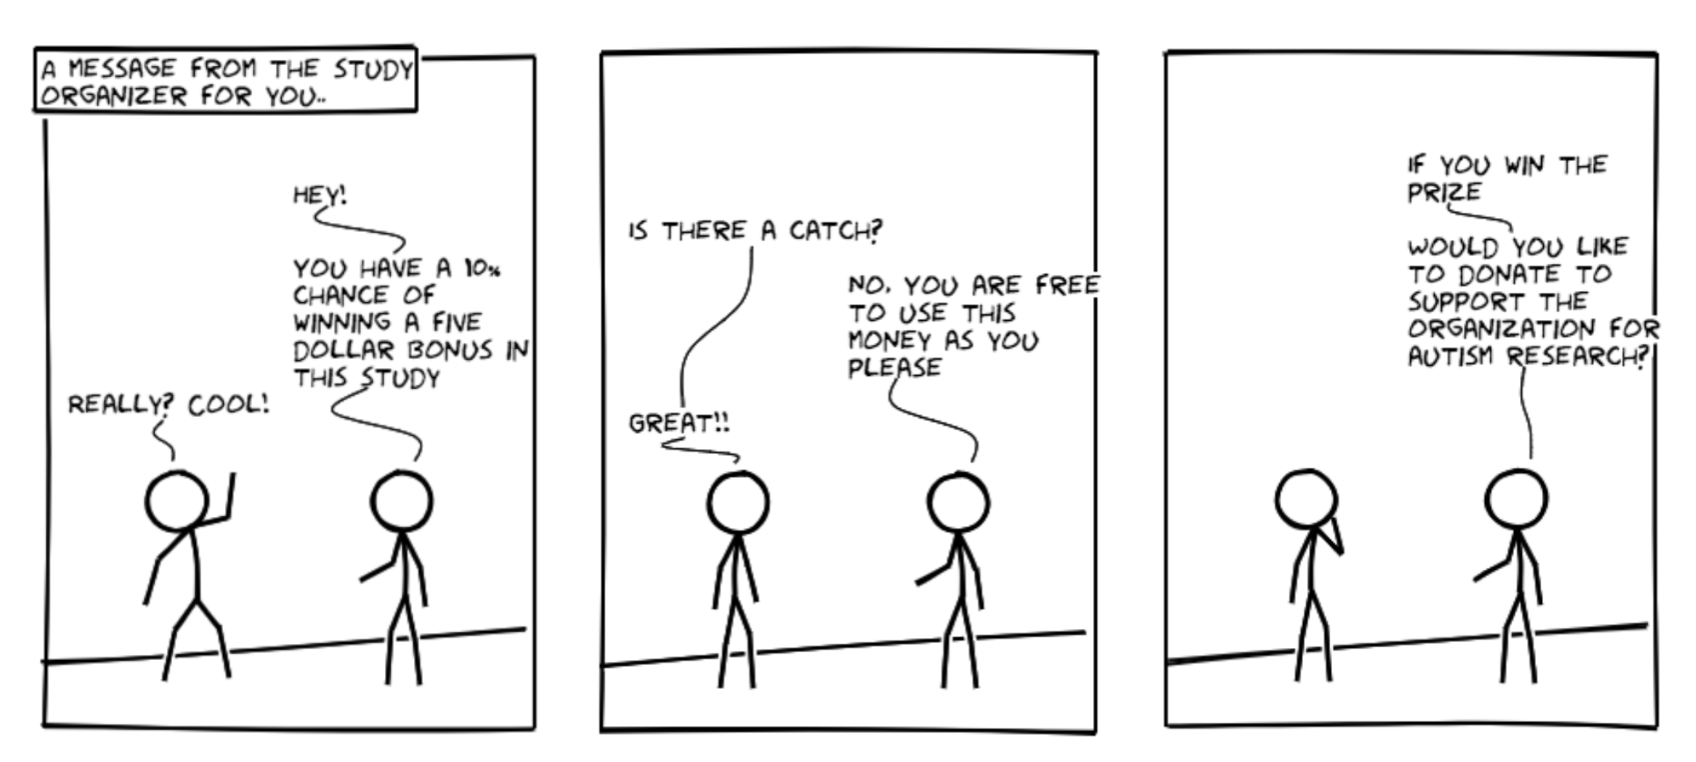
\includegraphics[width=\columnwidth]{./figures/abstract_comic.png}
	\caption{Messages in the abstract comic form}
	\label{fig:basic three comic panel}
\end{figure}

The objective of the persuasive message in all three conditions were the same, persuading participants to donate with a perspective bonus reward (10\% chance of winning \$5 bonus as additional compensation) to a charity.Study participant will be randomly assigned to one of the three conditions and make decision on the amount of donation based on their will.

\paragraph{Study Procedure} Once the participant consents to join the study, they will be asked if he/she is familiar with the Autism Spectrum Disorder (ASD). Then, participant will watch a short-video produced by the Organization for Autism Research that promotes its fundraising activity "RUN FOR AUTISM". After watch the video, participant will briefly summarize the video and provide their opinion about the effectiveness of the video, which is the task we mentioned in the recruiting message.

Then participants will be randomly assigned to each of the three conditions and read the persuasive message in different forms. In the message, the participant were provided a 10\% chance of winning \$ 5 additional compensation. They also have the opportunity to donate to the Autism Spectrum Disorder (ASD) which is the charity in the video they have watched before.

To best demonstrate the persuasiveness of the message itself, we diffused the responsibility of donation amount all the participants. So, before the participants make their decision, they will read "The total amount of money allocated to [the charity] by all the winning participants will be aggregated and donated at the end of the study."~\cite{lee2013does} Then the participants will be asked to decide the amount of money they were willing to donate on a slider bar with \$0 and \$5 as two ends. The default position of the slider bar is at \$0 end.

Before leaving the study, the participants were asked to fill demographic questions about their gender, age and education.

At the end of the study, we randomly chose 10 \% of the participants, donated to OAR based on those participants decision, and rewarded them.

To gather the basic statistics to create social proof, i.e.  X \% of participants donated in our study and validate the study procedure, we first ran a pilot study with two conditions, abstract-comic and pure-text before the actual experiment fielded.


\begin{figure}[bt]
	\centering
	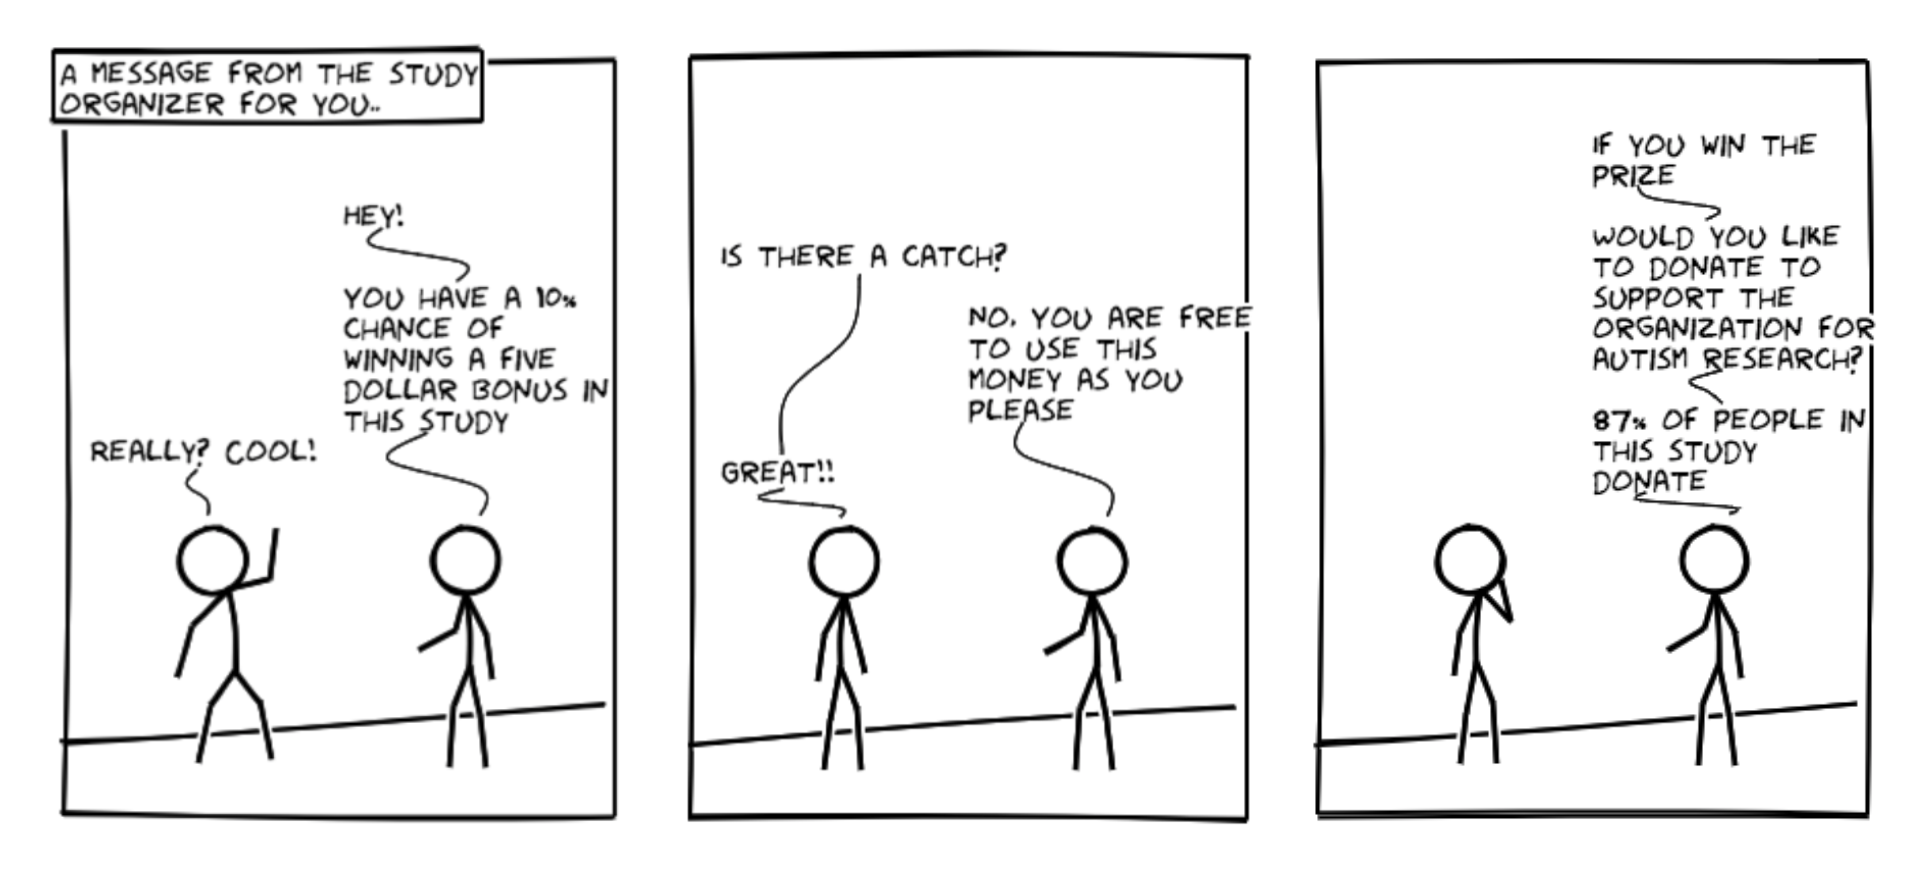
\includegraphics[width=\columnwidth]{./figures/social_proof.png}
	\caption{Messages with social proof.}
	\label{fig:basic three comic social proof}
\end{figure}

\paragraph{Organization for Autism Research (OAR)}
To increase the realism of our study, the donation decision is not hypothetical, participants will get the reward based on their decision and the donation will be made to, the Organization for Autism Research (OAR). We chose OAR as the charity in our study for two reasons, 1) The Autism Spectrum Disorder (ASD), a serious developmental disorder that impairs the communication and behavior, is a well-known disorder that can affect people in general. In other word, ASD is a problem potentially related to every participants in our study, which provides the basic interest for the participants to support related charitable organization and 2) the Organization for Autism Research is one of the most largest organization that helps individuals with autism and provides assistance to parents, families, teachers and caregivers. The goal of OAR is clear and reputable so participants won't question the authenticity of our message's motive.

\paragraph{Persuasive Messages}

The persuasive messages communicate three major objectives, 1) Participants will have 10 \% of chance winning \$ 5 bonus upon the completion of the study. 2) Participants are free to use the money as they please. and 3) Participants can donate this bonus to the Organization for Autism Research (OAR). Therefore, in the text condition, study participants will read the following message,
\begin{quote}
  \textit{You have a 10\% chance of winning a five dollar bonus in this study. You are free to use this money as you please. If you win the prize, would you like to donate to support the Organization for Autism Research?}
\end{quote}
In the two comic conditions, instead of creating a single panel comic as in the first study, we created three-panel comic strips to communicate the message. The three-panel comic strip allows us to leverage one of the most fascinating aspect of comics --- storytelling ~\cite{scott1993understanding}. Each of the three panel communicates one major objective in the message. The comic strip is created in the similar fashion as in the first study on preference. As we learned from the first study that appropriate gestures will maximize the persuasiveness of the comics, we then chose the gesture that we believe best suit for the scenario see~\Cref{fig:basic three comic panel}.

In the social-proof-comic condition, we created social-proof by adding one sentence on the last comic panel indicates the percentage of people in our study donated see~\Cref{fig:basic three comic social proof}. The percentage is based on number of people chose to donate in the pilot study.

% \begin{figure*}
%  \subfloat[Messages in the abstract comic form]{%
%   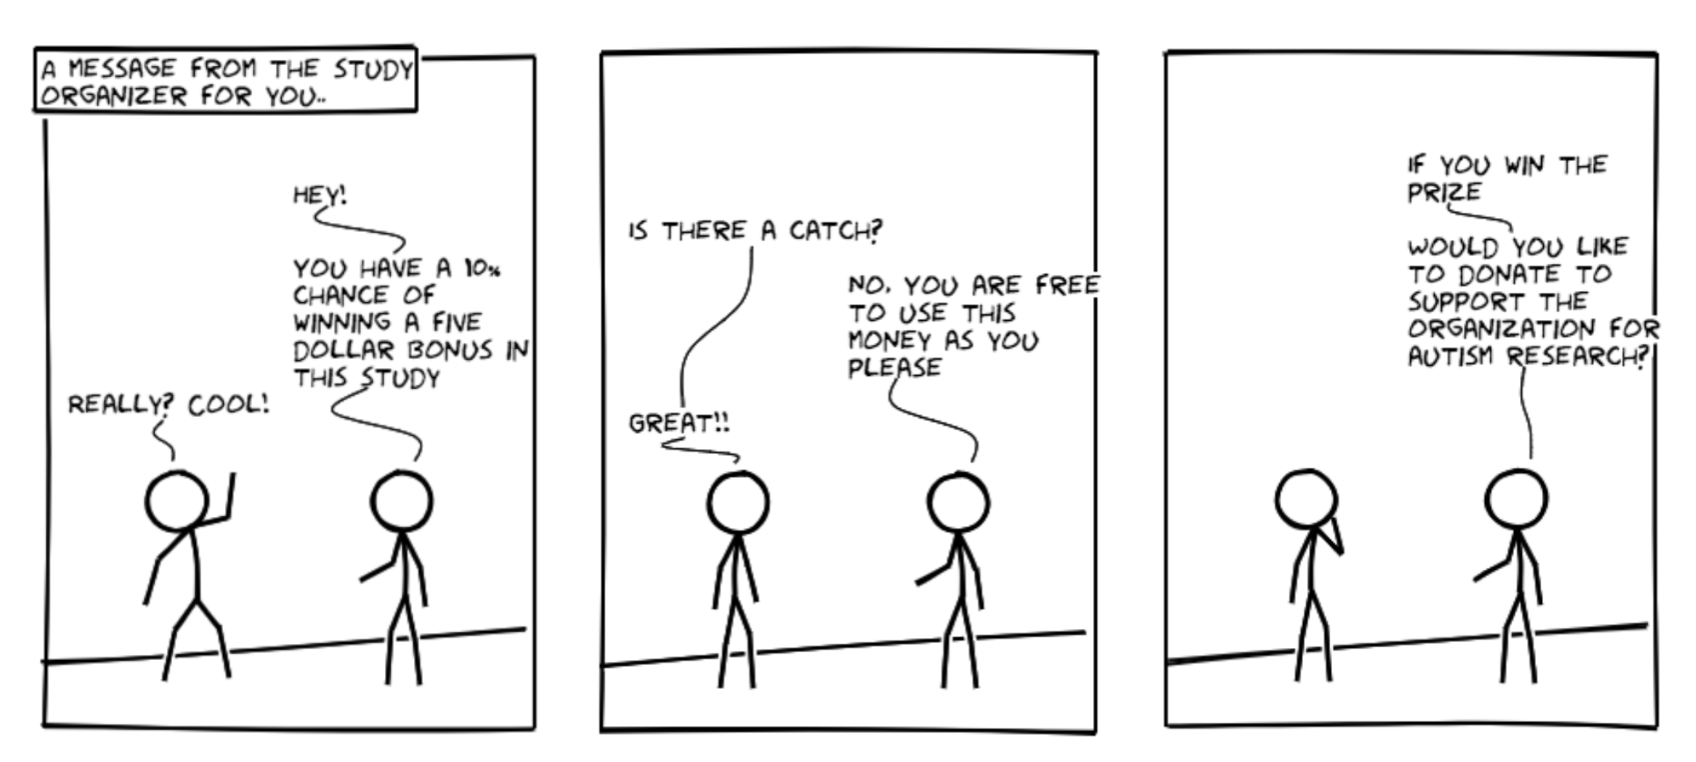
\includegraphics[width=0.5\textwidth]{./figures/abstract_comic.png}
%   } \hfill
%  \subfloat[Messages in the abstract comic form with social proof]{%
%   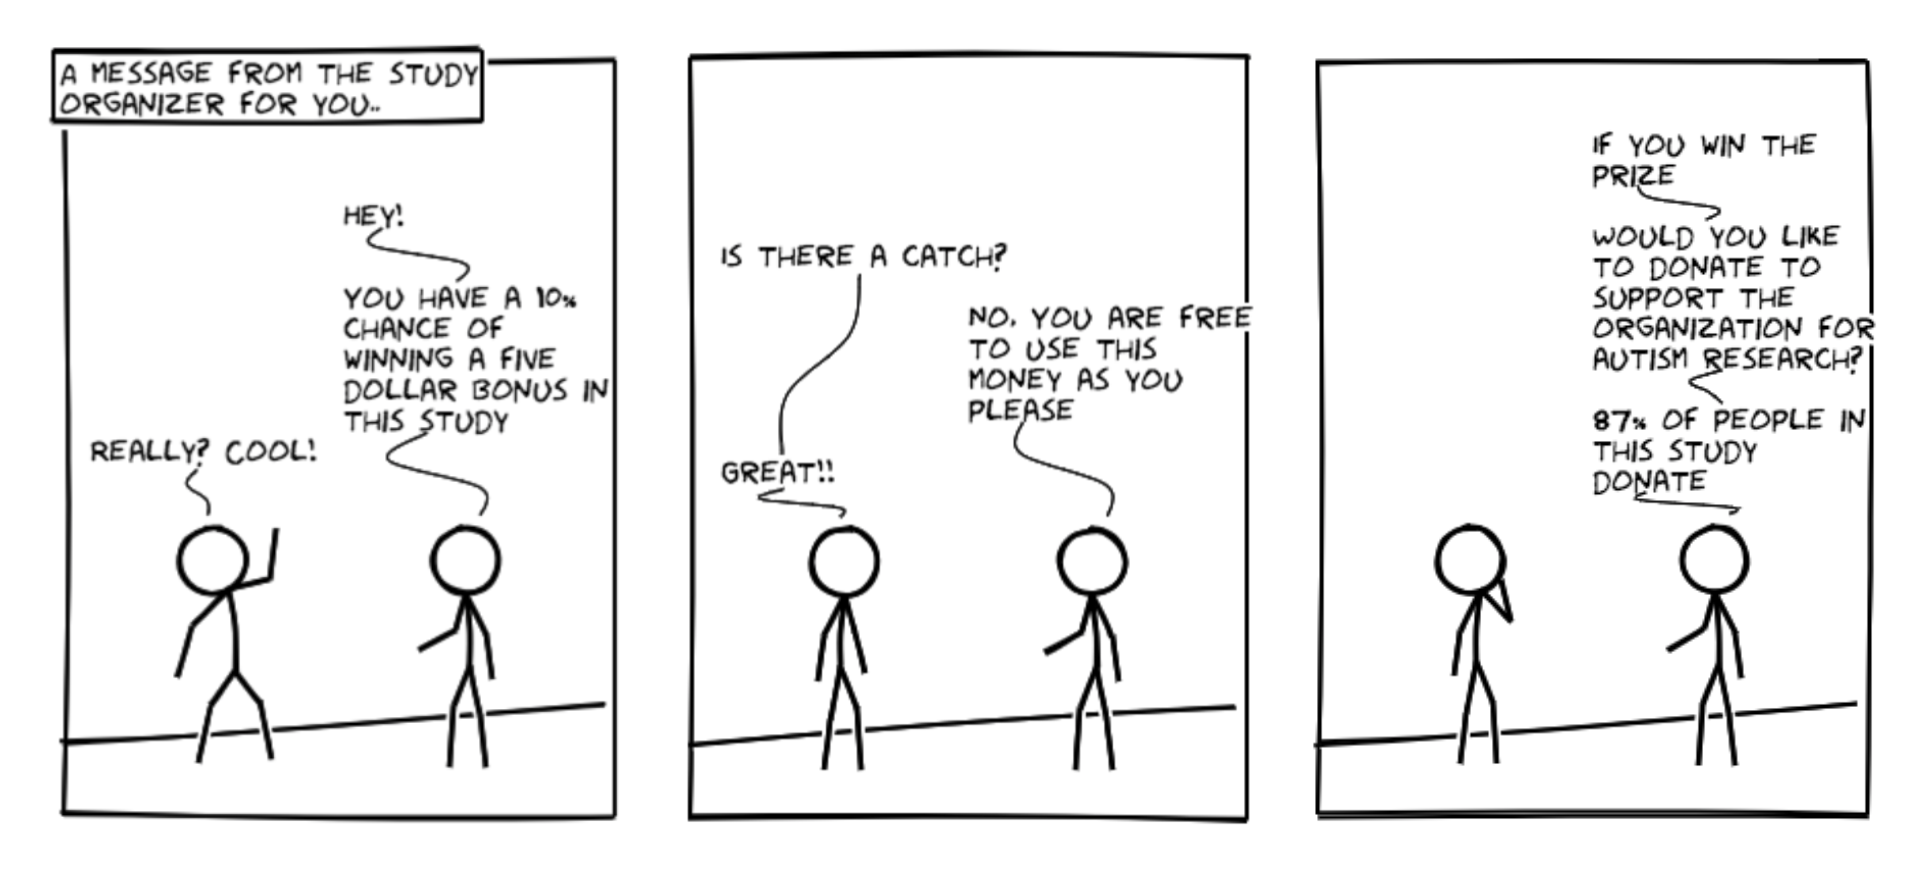
\includegraphics[width=0.5\textwidth]{./figures/social_proof.png}
%  }
%  \caption{The messages participants received in two abstract-comic conditions}
%  \label{fig:comic_messages_in_two_conditions}
% \end{figure*}

\subsubsection{Participants}
We published our HITs on Amazon Mechanical Turk titled with "A short survey about communicating autism campaign ads". Similar to the Study 1, the price tag is \$8/hr, the workers would get these rewards regardless of their performance, the threshold for participant to join was a 95\% Approval Rate. On the HIT page, and repeated responses will be rejected as instructed, participants would see a link to our experiment site and a text input box for them to enter a six-digit completion code.
